\documentclass{standalone}

\usepackage{pgfplots}
\usepgfplotslibrary{fillbetween}
\usepackage{lmodern}
\definecolor{deepskyblue3}{RGB}{0, 155, 206}

\begin{document}
{\hspace{0.15cm}
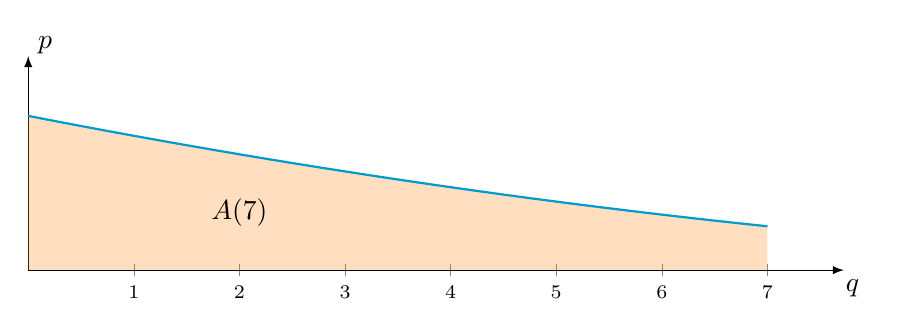
\begin{tikzpicture}

        
        \begin{axis}[
            width = 0.96\textwidth,
            height = 4cm,
            axis lines = middle,
            xmin = 0,
            xmax = 7.5,
            ymin = 0,
            ymax = 250,
            xtick = {1, 2, 3, 4, 5, 6, 7},
            % xticklabels = {$q_0$, $q_2$, $q^*$, $q_1$},
            scaled ticks = false,
            ytick = {\empty},
            % yticklabels = {$p_1$, $p^*$, $p_2$, $p_0$},
            ticklabel style = {font=\scriptsize},
            xlabel = $q$,
            ylabel = $p$,
            axis line style = {
                -latex,
                shorten >= -0.3cm,
                % shorten <=-12.5pt,
            },
            xlabel style={at={(ticklabel* cs:1)}, xshift = 0.2cm, anchor=north west},
            ylabel style={at={(ticklabel* cs:1)}, yshift = 0.2cm, anchor=south west},
        ]

            \addplot[name path = f, thick, deepskyblue3, samples = 51, smooth, domain = 0:7] {0.9*(x-15)^2};
            
            \path[name path = axis] (axis cs:0, 0) -- (axis cs: 7, 0);

             \addplot [
                thick,
                color = blue,
                fill = orange, 
                fill opacity = 0.25
            ]
            fill between[
                of = f and axis,
                soft clip = {domain = 0:7},
            ];

            \addplot[] coordinates {(2, 75)} node[] {${A(7)}$};
            
            
        \end{axis}

        \end{tikzpicture}
        }
\end{document}